\lipsum[3-8]

\begin{figure}
    \centering
    \begin{subfigure}[b]{0.3\textwidth}
        \centering
        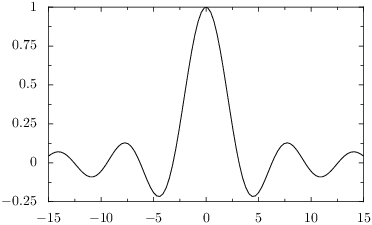
\includegraphics[width=\textwidth]{small_graph.png}
        \caption{$y=x$}
        \label{fig:y equals x}
    \end{subfigure}
    \hfill
    \begin{subfigure}[b]{0.3\textwidth}
        \centering
        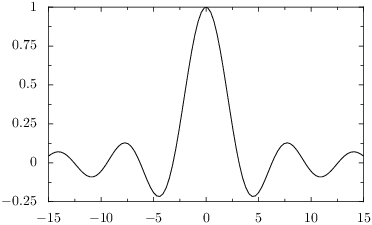
\includegraphics[width=\textwidth]{small_graph.png}
        \caption{$y=3sinx$}
        \label{fig:three sin x}
    \end{subfigure}
    \hfill
    \begin{subfigure}[b]{0.3\textwidth}
        \centering
        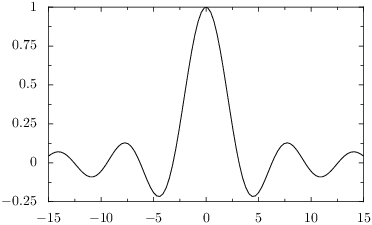
\includegraphics[width=\textwidth]{small_graph.png}
        \caption{$y=5/x$}
        \label{fig:five over x}
    \end{subfigure}
    \caption{Three simple graphs}
    \label{fig:three graphs}
\end{figure}

see \ref{fig:five over x}